\documentclass[12pt,aspectratio=169]{beamer}

% ====================================================
% ====================================================
% USEPACKAGES AND IMPORTS
% ====================================================
% ====================================================

\usepackage[T1]{fontenc}
\usepackage[utf8]{inputenc}
\usepackage[english]{babel}

% tables
\usepackage{tabularx}
\usepackage{colortbl}
\usepackage{multirow}
\usepackage{makecell}

% tikz and colors
\usepackage{tikz}
\usepackage{xcolor}
\usepackage{pgfplots}
\usepackage{pgfplotstable}
\usepackage{tikzsymbols}

\usetikzlibrary{calc}
\usetikzlibrary{trees}
\usetikzlibrary{patterns}
\usetikzlibrary{shadings}
\usetikzlibrary{positioning}
\usetikzlibrary{intersections}
\usepgfplotslibrary{patchplots}
\usepgfplotslibrary{fillbetween}
\usetikzlibrary{decorations.pathreplacing}

\usetikzlibrary{arrows}
\usetikzlibrary{arrows.meta}

\usetikzlibrary{shapes}
\usetikzlibrary{shapes.arrows}
\usetikzlibrary{shapes.callouts}
\usetikzlibrary{shapes.symbols}
\usetikzlibrary{shapes.geometric}

% boxes
\usepackage[many]{tcolorbox}

% math packages and fonts
\usepackage{bm}
\usepackage{ccfonts}
\usepackage{eulervm}
\usepackage{amsmath}
\usepackage{amsfonts}
\usepackage{amssymb}
\usepackage{amsthm}
\usepackage{mathtools}
\usepackage{nicefrac}
\usepackage{slashed}
\usepackage{bbold}
\usepackage{array}
\usepackage{cancel}

% algorithms and listings
\usepackage[ruled,vlined,linesnumbered]{algorithm2e}
\usepackage{listings}
\usepackage{setspace}

\tcbuselibrary{listings}
\tcbuselibrary{breakable}
\tcbuselibrary{skins}

% misc
\usepackage{soul}
\usepackage{pifont}
\usepackage{skull}
\usepackage{multicol}
\usepackage{animate}
\usepackage{hyperref}
\usepackage{wasysym}
\usepackage[absolute,overlay]{textpos}
\usepackage[hang,flushmargin]{footmisc}

% ====================================================
% ====================================================
% LAYOUT AND THEME
% ====================================================
% ====================================================

\usetheme{Copenhagen}

% color definitions
\definecolor{myblue1}{RGB}{35,119,189}
\definecolor{myblue2}{RGB}{95,179,238}
\definecolor{myblue3}{RGB}{129,168,207}
\definecolor{myblue4}{RGB}{26,89,142}

\definecolor{myred1}{RGB}{247,12,12}

% set theme colors
\setbeamercolor*{structure}{fg=myblue1,bg=blue}
\setbeamercolor*{palette primary}{use=structure,fg=white,bg=structure.fg}
\setbeamercolor*{palette secondary}{use=structure,fg=white,bg=structure.fg!75!black}
\setbeamercolor*{palette tertiary}{use=structure,fg=white,bg=structure.fg!50!black}
\setbeamercolor*{palette quaternary}{fg=black,bg=white}

\setbeamertemplate{itemize item}[circle]
\setbeamertemplate{itemize subitem}[circle]
\setbeamertemplate{itemize subsubitem}[circle]

\setbeamertemplate{enumerate item}[circle]
\setbeamertemplate{enumerate subitem}[circle]
\setbeamertemplate{enumerate subsubitem}[circle]

\setbeamercolor{itemize item}{fg=myblue1}
\setbeamercolor{itemize subitem}{fg=myblue1}
\setbeamercolor{itemize subsubitem}{fg=myblue1}

\setbeamertemplate{section in toc}[circle]
\setbeamertemplate{subsection in toc}[circle]
\setbeamerfont{subsection in toc}{size=\scriptsize}

\setbeamercolor{frametitle continuation}{fg=black}

% title graphic -- sap logo and dhbw logo
\titlegraphic{
\includegraphics[scale=0.1]{../03_img/logo_sap}\hspace*{4.75cm}~%
   	
\includegraphics[scale=0.05]{../03_img/logo_dhbw}
}

\makeatletter
% frame title
\defbeamertemplate*{frametitle}{mydefault}[1][left]
{
  	\ifbeamercolorempty[bg]{frametitle}{}{\nointerlineskip}%
  	\nointerlineskip%
 	\@tempdima=\textwidth%
  	\advance\@tempdima by\beamer@leftmargin%
  	\advance\@tempdima by\beamer@rightmargin%
  	\begin{tcolorbox}[
  		enhanced,
  		outer arc=0pt,
  		arc=0pt,
  		boxrule=0pt,
  		top=0pt,
  		bottom=0pt,
  		enlarge left by=-\beamer@leftmargin,
  		enlarge right by=-\beamer@rightmargin,
  		width=\paperwidth,
  		nobeforeafter,
  		interior style={
    			left color=myblue2,
    			right color=white
    		},
  		shadow={0mm}{-0.4mm}{0mm}{black!60,opacity=0.6},    
  		shadow={0mm}{-0.8mm}{0mm}{black!40,opacity=0.4},    
  	]
    	\usebeamerfont{frametitle}%
    	\vbox{}\vskip-1ex%
    	\if@tempswa\else\csname beamer@fte#1\endcsname\fi%
    	\insertframetitle\par%
    	{%
      		\ifx\insertframesubtitle\@empty%
      		\else%
      		{\usebeamerfont{framesubtitle}\usebeamercolor[fg]{black}\insertframesubtitle\strut\par}%
      		\fi
    	}%
    	\vskip-1ex%
    	\if@tempswa\else\vskip-.3cm\fi
  	\end{tcolorbox}%
}

% footline of a frame
\defbeamertemplate*{footline}{mysplit theme}
{%
  	\leavevmode%
  	\hbox{
		\begin{beamercolorbox}[
			wd=.5\paperwidth,ht=2.5ex,dp=1.125ex,leftskip=.3cm plus1fill,rightskip=.3cm
		]{author in head/foot}%
    			\usebeamerfont{author in head/foot}\insertshortauthor\ (\insertinstitute), \insertdate
  		\end{beamercolorbox}%
  		\begin{beamercolorbox}[
			wd=.5\paperwidth,ht=2.5ex,dp=1.125ex,leftskip=.3cm,rightskip=.3cm plus1fil
		]{title in head/foot}%
    			\usebeamerfont{title in head/foot}\insertshorttitle\hfill
    			\insertprefix-\insertframenumber/\inserttotalframenumber\hspace*{0.5em}
  		\end{beamercolorbox}}%
  	\vskip0pt%
}
\makeatother

% ====================================================
% ====================================================
% COMMANDS AND GENERAL DEFINITIONS
% ====================================================
% ====================================================

% page number prefix
\newcommand\insertprefix{}  % empty by default
\newcommand\prefix[1]{\renewcommand\insertprefix{#1}}

% math definitions
% ====================================================
\DeclareMathOperator*{\argmax}{arg\,max}
\DeclareMathOperator*{\argmin}{arg\,min}
\newcommand*\diff{\mathop{}\!\mathrm{d}}

\newcommand*{\vertbar}{\rule[-1ex]{0.5pt}{2.5ex}}
\newcommand*{\horzbar}{\rule[.5ex]{2.5ex}{0.5pt}}

% commands
% ====================================================

% highlight commands
% --------------------------------------------------------------------------------------------------------
% highlight command
\newcommand{\highlight}[1]{\textcolor{myblue1}{\textbf{#1}}}
\newcommand{\highlighttt}[1]{\textcolor{myblue1}{\texttt{#1}}}
\newcommand{\Highlight}[1]{\textcolor{myred1}{\textbf{#1}}}

% blue color boxes (with frame/without frame/without fill)
\newtcolorbox{boxBlue}{colback=myblue1!10!white,colframe=myblue4}
\newtcolorbox{boxBlueNoFrame}{colback=myblue1!10!white,colframe=myblue1!10!white}
\newtcolorbox{boxBlueNoFill}{colback=white,colframe=myblue4}

% font commands
% --------------------------------------------------------------------------------------------------------
\newcommand{\linkstyle}[1]{\underline{\smash{\texttt{#1}}}} 		% style of hyperlinks

% tikz commands
% --------------------------------------------------------------------------------------------------------

% yellow sticky note
\newcommand{\bubble}[3]{
\begin{textblock}{100}(#1, #2)
      	\begin{tikzpicture}
		\node[rectangle,draw=yellow,very thick,fill=yellow!60,align=center] at (0,0) {#3};
	\end{tikzpicture}
\end{textblock}
}

\newcommand{\floattext}[3]{
\begin{textblock}{100}(#1, #2)
      	#3
\end{textblock}
}

\newcommand{\doublecircle}[2]{
	\draw[fill=white,draw=myblue1] (#1,#2) circle (2mm);
	\draw[fill=myblue1,draw=myblue1] (#1,#2) circle (1.5mm);
}

% slide modifiers
% --------------------------------------------------------------------------------------------------------
% mark slide as optional
\newcommand{\optional}{
	\begin{textblock}{100}(0.15,0.30)
      		
\includegraphics[scale=0.2]{../03_img/scream}
    	\end{textblock}
}

% mark slide as important
\newcommand{\important}{
	\begin{textblock}{100}(0.10,0.15)
      		
\includegraphics[scale=0.1]{../03_img/important}
    	\end{textblock}
}

% citation
% --------------------------------------------------------------------------------------------------------
% first argument in {book, online, article}
\newcommand{\literature}[5]{
	\setbeamertemplate{bibliography item}[#1]
	\bibitem{#2}
	\highlight{#3} \\
	\textcolor{darkgray}{\textit{#4}} \\
	\textcolor{black}{#5}
}
% cite content
\newcommand{\citeAuthor}[3]{\vfill\scriptsize\textcolor{lightgray}{#1 \cite{#2} #3}}

% slide architecture
% --------------------------------------------------------------------------------------------------------
% divide frame into two parts
\newcommand{\divideTwo}[4]{
	\begin{minipage}{#1\textwidth}
		#2
	\end{minipage}
	\hfill
	\begin{minipage}{#3\textwidth}
		#4
	\end{minipage}
}

% divide frame into two parts (start on top)
\newcommand{\divideTwoTop}[4]{
	\begin{minipage}[t]{#1\textwidth}
		#2
	\end{minipage}
	\hfill
	\begin{minipage}[t]{#3\textwidth}
		#4
	\end{minipage}
}

% special pages
% --------------------------------------------------------------------------------------------------------
% title page
\newcommand{\maketitlepage}{
	{
		\beamertemplatenavigationsymbolsempty
		\usebackgroundtemplate{%
			\tikz[overlay,remember picture] \node[opacity=0.2, at=(current page.center)] {
  				
\includegraphics[height=\paperheight,width=\paperwidth]{../03_img/processor.jpg}
			};
		}
		\begin{frame}[plain]
			\vspace*{0.75cm}
			\maketitle
			\vfill
			\begin{center}
				\footnotesize Find all slides on \href{https://github.com/DaWe1992/Applied_ML_Fundamentals}{\linkstyle{GitHub}}
			\end{center}
		\end{frame}
	}
}

% divider page
\newcommand{\makedivider}[1]{
	{
		\beamertemplatenavigationsymbolsempty
		\usebackgroundtemplate{%
			\tikz[overlay,remember picture] \node[opacity=0.2, at=(current page.center)] {
  				
\includegraphics[height=\paperheight,width=\paperwidth]{../03_img/processor.jpg}
			};
		}
		\begin{frame}[plain]
			\vfill
			\begin{boxBlue}
				\centering
				\textbf{Section:} \\
				\large \highlight{#1}
			\end{boxBlue}
			\vfill
			\centering
			
\includegraphics[scale=0.05]{../03_img/logo_dhbw.png}
			\vfill
		\end{frame}
	}
}

% overview page
\newcommand{\makeoverview}[1]{
	\begin{frame}{Lecture Overview}{}
		\begin{tabbing}
			\hspace*{3.5cm}\= \kill
			\ifnum #1=1 \highlight{\textbf{Unit I:}} \else \textbf{Unit I:} \fi
			\> \ifnum #1=1 \highlight{Machine Learning Introduction} \else Machine Learning Introduction \fi \\
		\end{tabbing}
	\end{frame}
}

% thank you page
\newcommand{\makethanks}{
	{\beamertemplatenavigationsymbolsempty
	\begin{frame}[plain]
		\vfill
		\begin{boxBlue}
			\centering
			\Large \highlight{Thank you very much for the attention!}
		\end{boxBlue}
		
		\vfill\footnotesize
		\begin{tabbing}
			\hspace*{1.5cm}\= \kill
			\highlight{Topic:} 	\> \inserttitle \\
			\highlight{Date:} 	\> \insertdate
		\end{tabbing}
		
		\vfill
		\highlight{Contact:} \\
		\insertauthor\ (D062271) \\
		\insertinstitute \\
		\href{mailto:daniel.wehner@sap.com}{\linkstyle{daniel.wehner@sap.com}}
		
		\vfill\normalsize
		\begin{center}
			\large\highlight{Do you have any questions?}
		\end{center}
		\vfill
	\end{frame}}
}

% global pfgplots settings
% --------------------------------------------------------------------------------------------------------
\pgfplotsset{
	% allow filtering of data for pgfplots
	discard if/.style 2 args={
        		x filter/.code={
            		\edef\tempa{\thisrow{#1}}
            		\edef\tempb{#2}
            		\ifx\tempa\tempb
                		\def\pgfmathresult{inf}
            		\fi
        		}
    	},
    	discard if not/.style 2 args={
        		x filter/.code={
            		\edef\tempa{\thisrow{#1}}
            		\edef\tempb{#2}
            		\ifx\tempa\tempb
            		\else
                		\def\pgfmathresult{inf}
            		\fi
        		}
    	}
}


% ====================================================
% ====================================================
% PRESENTATION DATA
% ====================================================
% ====================================================

\title[Decision Theory]{*** Applied Machine Learning Fundamentals *** Bayesian Decision Theory}
\institute{SAP\,SE}
\author{M.\,Sc. Daniel Wehner}
\date{Winter term 2019/2020}
\prefix{BDT}

% ====================================================
% ====================================================
% BEGIN OF DOCUMENT
% ====================================================
% ====================================================

\begin{document}

% Title frame
%______________________________________________________________________
\maketitlepage


% Lecture Overview
%______________________________________________________________________
\begin{frame}{Lecture Overview}{}
	\makeoverview{3}
\end{frame}


% Agenda
%______________________________________________________________________
\begin{frame}{Agenda for this Unit}
	\begin{multicols}{2}
		\tableofcontents
	\end{multicols}
\end{frame}


% Section: Bayesian Decision Theory
%______________________________________________________________________
\section{Bayesian Decision Theory}
\makedivider{Bayesian Decision Theory}

% Subsection: Introduction
% --------------------------------------------------------------------------------------------------------
\subsection{Introduction}

% Statistical Methods
\begin{frame}{Statistical Methods}{}
	\begin{itemize}
		\item Statistical methods assume that the process that `generates' the data is governed by the
			\highlight{rules of probability}
		\item The data is understood to be a set of \highlight{random samples} from some
			underlying \highlight{probability distribution}
		\item This is the reason for the name \highlight{statistical machine learning}
	\end{itemize}
	\begin{boxBlueNoFrame}
		The basic assumption about how the data is generated is always there, even if you don't see
		a single probability distribution!
	\end{boxBlueNoFrame}
\end{frame}


% Running Example: Optical Character Recognition (OCR)
\begin{frame}{Running Example: Optical Character Recognition (OCR)}{}
	\begin{figure}
		\centering
		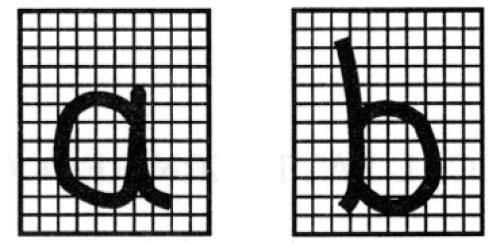
\includegraphics[scale=0.6]{03_decision_theory/02_img/characters}
	\end{figure}
	\vspace*{-1mm}
	\footnotesize
	\Highlight{Goal: Classify a new letter so that the probability of a wrong classification is minimized}
\end{frame}


% Subsection: Class Conditional Probabilities
% --------------------------------------------------------------------------------------------------------
\subsection{Class Conditional Probabilities}

% Class Conditional Probabilities
\begin{frame}{Class Conditional Probabilities}{}
	\begin{itemize}
		\item First concept: \highlight{Class conditional probabilities}
		\item Probability of $\bm{x}$ given a specific class $\mathcal{C}_k$ is formally written as:
		\begin{equation}
			p(\bm{x} \vert \mathcal{C}_k) \in [0, 1]
		\end{equation}
		\item $\bm{x} \in \mathbb{R}^m$ is a feature vector, e.\,g. \#\,black pixels, height-width ratio, ...
		\begin{figure}
			\centering
			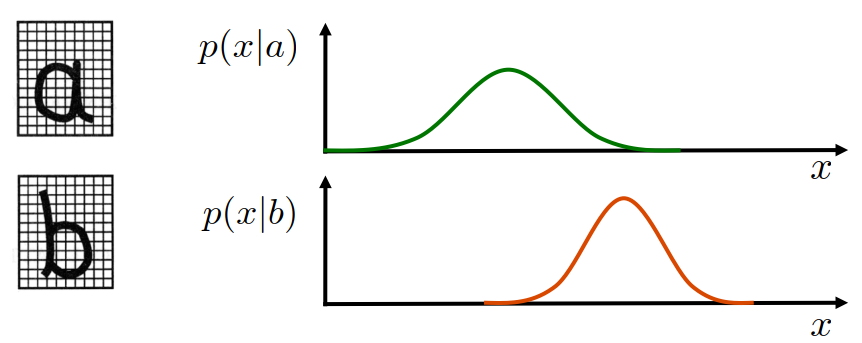
\includegraphics[scale=0.3]{03_decision_theory/02_img/conditional_probabilities}
		\end{figure}
	\end{itemize}
\end{frame}


% Class Conditional Probabilities (Ctd.)
\begin{frame}{Class Conditional Probabilities (Ctd.)}{}
	\divideTwo{0.49}{
		\begin{figure}
			\centering
			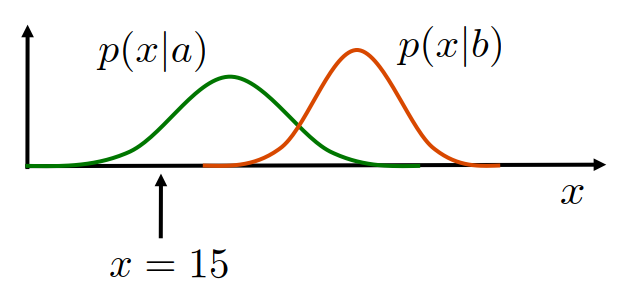
\includegraphics[scale=0.4]{03_decision_theory/02_img/conditional_probabilities_overlap1}
		\end{figure}
	}{0.49}{
		\begin{figure}
			\centering
			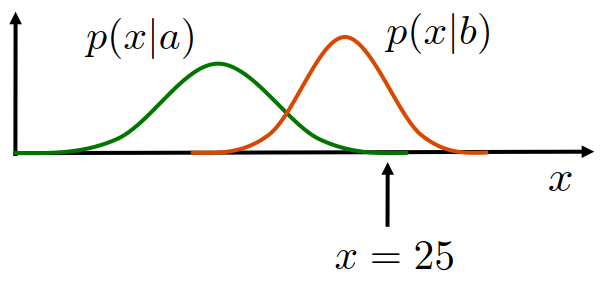
\includegraphics[scale=0.4]{03_decision_theory/02_img/conditional_probabilities_overlap2}
		\end{figure}
	}
	\vspace*{3mm}
	\begin{boxBlueNoFrame}
		If $\bm{x} = 15$ we would predict class $a$ since $p(15 \vert a) > p(15 \vert b)$. \\
		If $\bm{x} = 25$ we would output class $b$ since $p(25 \vert b) > p(25 \vert a)$.
	\end{boxBlueNoFrame}
\end{frame}


% Class Conditional Probabilities (Ctd.)
\begin{frame}{Class Conditional Probabilities (Ctd.)}{}
	\bubble{12}{5}{
		\scriptsize We have a problem!
	}
	\begin{figure}
		\centering
		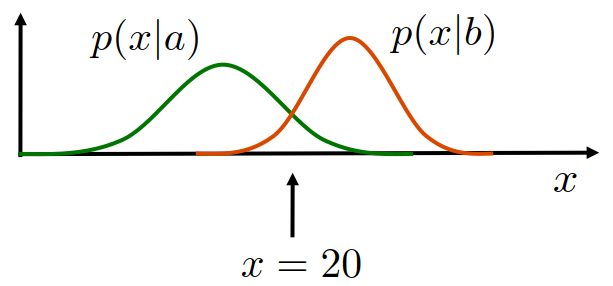
\includegraphics[scale=0.5]{03_decision_theory/02_img/conditional_probabilities_overlap3}
	\end{figure}
	\vspace*{-3mm}
	\begin{itemize}
		\item \highlight{Which class should be chosen now?}
		\item The conditional probabilities are the same... $\skull$
	\end{itemize}
\end{frame}


% Subsection: Class Priors
% --------------------------------------------------------------------------------------------------------
\subsection{Class Priors}

% Class Prior Probabilities
\begin{frame}{Class Prior Probabilities}{}
	\bubble{10}{10}{
		\footnotesize How would you decide now?
	}
	\begin{itemize}
		\item Second concept: \highlight{Class priors}
		\item The prior probability of a data point belonging to a particular class $\mathcal{C}$
		\begin{alignat*}{2}
			\mathcal{C}_1 &\equiv a \qquad p(\mathcal{C}_1) &&= 0.75 \\
			\mathcal{C}_2 &\equiv b \qquad p(\mathcal{C}_2) &&= 0.25
		\end{alignat*}
		\item By definition:
		\begin{itemize}
			\item $0 \le p(\mathcal{C}_k) \le 1,\ \forall k$
			\item The sum of all probabilities equals one: $\sum_{k=1}^{\vert \mathcal{C} \vert} p(\mathcal{C}_k) = 1$
		\end{itemize}
		\item \highlight{The class prior is equivalent to a prior belief in the class label}
	\end{itemize}
\end{frame}


% How to get the Prior Probabilities?
\begin{frame}{How to get the Prior Probabilities?}{}
	\bubble{11}{5.25}{
		\footnotesize But don't count apples!
	}
	\vspace*{4mm}
	\begin{figure}
		\centering
		
\includegraphics[scale=0.6]{03_decision_theory/02_img/count_count_bubble}
	\end{figure}
	\begin{textblock}{100}(4,4.5)
		\footnotesize \highlight{Count Count's advice:}
	\end{textblock}
	\begin{textblock}{100}(4,6.25)
		\textbf{Simply count the} \\
		\textbf{number of instances} \\
		\textbf{in each class!}
	\end{textblock}
\end{frame}


% Subsection: Bayes' Theorem
% --------------------------------------------------------------------------------------------------------
\subsection{Bayes' Theorem}

% Bayes' Theorem
\begin{frame}{Bayes' Theorem}{}\important
	\begin{itemize}
		\item What we actually want to compute: $P(\mathcal{C}_k \vert \bm{x}) \Rightarrow$
			\highlight{Posterior probability}
		\item We can compute it by applying \highlight{Bayes' theorem}
		\item This is one of the \Highlight{most important formulas (!!!)}
	\end{itemize}

	\begin{boxBlue}
		\begin{equation}
			\overbracket{p(\mathcal{C}_k \vert \bm{x})}^{\text{\highlight{Class posterior}}}
				= \frac{
					\overbracket{p(\bm{x} \vert \mathcal{C}_k)}^{\text{\highlight{Class cond.}}}
					\cdot
					\overbracket{p(\mathcal{C}_k)}^{\text{\highlight{Class prior}}}
				}{
					\underbracket{p(\bm{x})}_{\text{\highlight{Normalization term}}}
				}
				= \frac{
					p(\bm{x} \vert \mathcal{C}_k) \cdot p(\mathcal{C}_k)
				}{
					\sum_{j=1}^{\vert \mathcal{C} \vert} p(\bm{x} \vert \mathcal{C}_j) \cdot p(\mathcal{C}_j)
				}
		\end{equation}
	\end{boxBlue}
\end{frame}


% Calculation of the Posterior Probability
\begin{frame}{Calculation of the Posterior Probability}{}
	\divideTwo{0.49}{
		\footnotesize
		\begin{itemize}
			\item By applying Bayes' theorem we can compute the posterior
			\item Simply plug \ding{182} and \ding{183} into Bayes' theorem
			\begin{enumerate}
				\item Class prior probabilities
				\item Class conditional probabilities
			\end{enumerate}
		\end{itemize}
		\begin{boxBlueNoFrame}
			We get the final \highlight{decision boundary}
		\end{boxBlueNoFrame}
	}{0.45}{
		\begin{figure}
			\centering
			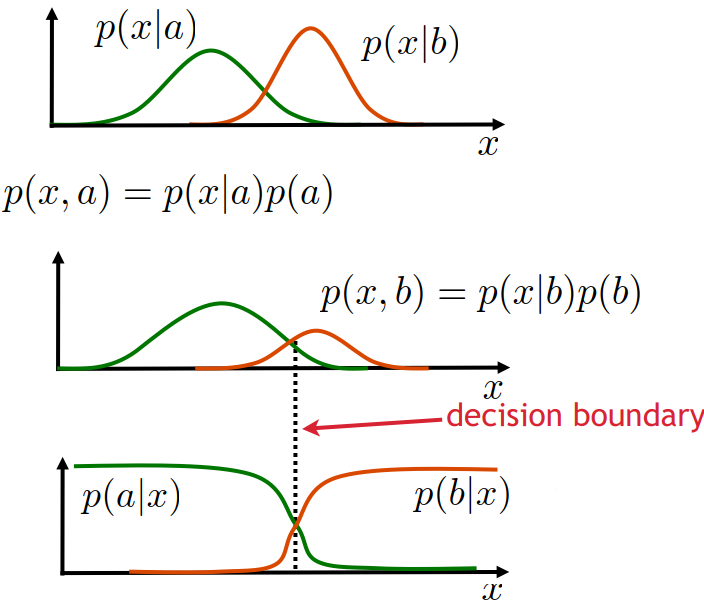
\includegraphics[scale=0.3]{03_decision_theory/02_img/decision_boundary}
		\end{figure}
	}
\end{frame}


% Subsection: Bayes' optimal Classifier
% --------------------------------------------------------------------------------------------------------
\subsection{Bayes' optimal Classifier}

% Error Minimization
\begin{frame}{Error Minimization}{}
	\divideTwo{0.45}{
		\begin{figure}
			\centering
			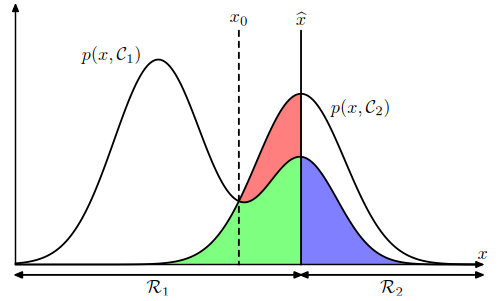
\includegraphics[scale=0.5]{03_decision_theory/02_img/error_minimization}
		\end{figure}
	}{0.49}{
		\begin{align*}
			p(error) 
				&= p(x \in \mathcal{R}_1, \mathcal{C}_2) + p(x \in \mathcal{R}_2, \mathcal{C}_1) \\
				&= \overbracket{
						\int_{\mathcal{R}_1} p(x \vert \mathcal{C}_2) \cdot p(\mathcal{C}_2) \diff x
					}^{\text{\textcolor{red}{red} + \textcolor{green!80!black}{green} area}}\ + \\
				&\phantom{=}\ \underbracket{
						\int_{\mathcal{R}_2} p(x \vert \mathcal{C}_1) \cdot p(\mathcal{C}_1) \diff x
					}_{\text{\textcolor{blue}{blue} area}}
		\end{align*}
	}
\end{frame}


% Bayes' optimal Classifier
\begin{frame}{Bayes' optimal Classifier}{}\important
	\begin{itemize}
		\item Decision rule:
		\begin{itemize}
			\item Decide $\mathcal{C}_1$ if $p(\mathcal{C}_1 \vert \bm{x}) > p(\mathcal{C}_2 \vert \bm{x})$
			\item This is equivalent to: \textit{(we don't need the normalization)}
			\begin{equation}
				p(\bm{x} \vert \mathcal{C}_1) \cdot p(\mathcal{C}_1) >
					p(\bm{x} \vert \mathcal{C}_2) \cdot p(\mathcal{C}_2)
			\end{equation} 
			\item Which is in turn equivalent to:
			\begin{equation}
				\frac{p(\bm{x} \vert \mathcal{C}_1)}{p(\bm{x} \vert \mathcal{C}_2)} >
					\frac{p(\mathcal{C}_2)}{p(\mathcal{C}_1)}
			\end{equation}
		\end{itemize}
		\item A classifier obeying this rule is called \highlight{Bayes' optimal Classifier}
	\end{itemize}
\end{frame}


% Section: Na\"{i}ve Bayes Classifier
%______________________________________________________________________
\section{Na\"{i}ve Bayes Classifier}
\makedivider{Na\"{i}ve Bayes Classifier}

% Subsection: Assumptions and Algorithm
% --------------------------------------------------------------------------------------------------------
\subsection{Assumptions and Algorithm}

% A na\"{i}ve Assumption
\begin{frame}{A na\"{i}ve Assumption}{}
	\bubble{12}{4.25}{
		\scriptsize Our first classification \\[-2mm]
		\scriptsize algorithm!
	}
	\begin{itemize}
		\item We want to compute $p(\mathcal{C}_k \vert \bm{x})$. Recall Bayes' theorem:
		\begin{equation}
			p(\mathcal{C}_k \vert \bm{x}) = \frac{p(\bm{x} \vert \mathcal{C}_k) \cdot p(\mathcal{C}_k)}{p(\bm{x})}
		\end{equation}
		\item Assumptions:
		\begin{itemize}
			\item All $x_i \in \bm{x}$ are \highlight{pairwise conditionally independent}
				($\Rightarrow$ \textbf{na\"{i}ve})
			\begin{equation}
				p(\bm{x} \vert \mathcal{C}_k) 
					= p(x_1 \vert \mathcal{C}_k) \cdot p(x_2 \vert \mathcal{C}_k, x_1) \cdot
						p(x_3 \vert \mathcal{C}_k, x_1, x_2) \cdot ... 
					= \prod_{j=1}^m p(x_j \vert \mathcal{C}_k)
			\end{equation}
			\item $p(\bm{x})$ is constant w.\,r.\,t. class label
				$\Rightarrow$ \highlight{It is omitted}
		\end{itemize}
	\end{itemize}
\end{frame}


% How to get the most probable Class?
\begin{frame}{How to get the most probable Class?}{}\important
	\bubble{1}{12}{
		\scriptsize $\widehat{p}$ denotes an \\[-2mm]
		\scriptsize \textbf{approximated} probability
	}
	\begin{itemize}
		\item \textbf{Given:}
		\begin{itemize}
			\item New instance $\bm{x} = \langle x_1, x_2, \dots, x_m \rangle$ to be classified
			\item Finite set of $\kappa$ classes $\{ \mathcal{C}_1, \mathcal{C}_2, \dots, \mathcal{C}_{\kappa} \}$
			\item \highlight{Labeled} training data ($\Rightarrow$ supervised learning)
		\end{itemize}
		\item \textbf{Wanted:} Most probable class $\mathcal{C}_{MAP}$ (maximum aposteriori) for $\bm{x}$:
		\begin{align}
			\mathcal{C}_{MAP}
				&= \argmax_{\mathcal{C}_k \in \{ \mathcal{C}_1, \dots, \mathcal{C}_{\kappa} \}} 
					\widehat{p}(\mathcal{C}_k \vert \bm{x}) \\
				&= \argmax_{\mathcal{C}_k \in \{ \mathcal{C}_1, \dots, \mathcal{C}_{\kappa} \}} 
					\widehat{p}(\mathcal{C}_k) \prod_{j=1}^m \widehat{p}(x_j \vert \mathcal{C}_k)
		\end{align}
	\end{itemize}
\end{frame}


% How to get the most probable Class? (Ctd.)
\begin{frame}{How to get the most probable Class? (Ctd.)}{}
	\vspace*{-2mm}
	\begin{figure}
	\centering
	\begin{tikzpicture}[
		scale=0.6,
		every node/.style={scale=0.9}
	]

		% draw rectangles
		\draw[ultra thick] (0,0) rectangle (3,8);
		\draw[ultra thick] (4,0) rectangle (11,8);
		\draw[ultra thick] (12,0) rectangle (15,8);

		\node at (1.5,8.5) {\footnotesize{Apriori Probabilities}};
		\node at (7.5,8.5) {\footnotesize{Feature Contributions}};
		\node at (13.5,8.5) {\footnotesize{Aposteriori Probabilities}};

		\node at (3.5,4) {x};
		\node at (7.5,4) {x ... x};
		\node at (11.5,4) {=};
	
		% first coordinate system
		\node at (1.5,4) {
			\begin{tikzpicture}[scale=0.7]
				\node at (1.5,8) {\footnotesize{$p(\mathcal{C}_k)$}};
		
				\draw[fill=red!30,draw=red,thick] (0.8,3) rectangle (1.2,6.2);
				\draw[fill=blue!30,draw=blue,thick] (1.4,3) rectangle (1.8,5.8);
				\draw[fill=green!30,draw=green,thick] (2.0,3) rectangle (2.4,6.9);

				\draw[thick] (0.5,3) -- (2.5,3);
				\draw[thick] (0.5,3) -- (0.5,7);

				\node[rotate=90] at (1.0,2.0) {\footnotesize{Class 1}};
				\node[rotate=90] at (1.6,2.0) {\footnotesize{Class 2}};
				\node[rotate=90] at (2.2,2.0) {\footnotesize{Class 3}};
			\end{tikzpicture}
		};

		% second coordinate system
		\node at (5.5,4) {
			\begin{tikzpicture}[scale=0.7]
				\node at (1.5,8) {\footnotesize{$p(x_1 \vert \mathcal{C}_k)$}};

				\draw[fill=red!30,draw=red,thick] (0.8,3) rectangle (1.2,4.2);
				\draw[fill=blue!30,draw=blue,thick] (1.4,3) rectangle (1.8,4.0);
				\draw[fill=green!30,draw=green,thick] (2.0,3) rectangle (2.4,3.5);

				\draw[thick] (0.5,3) -- (2.5,3);
				\draw[thick] (0.5,3) -- (0.5,7);

				\node[rotate=90] at (1.0,2.0) {\footnotesize{Class 1}};
				\node[rotate=90] at (1.6,2.0) {\footnotesize{Class 2}};
				\node[rotate=90] at (2.2,2.0) {\footnotesize{Class 3}};
			\end{tikzpicture}
		};

		% third coordinate system
		\node at (9.5,4) {
			\begin{tikzpicture}[scale=0.7]
				\node at (1.5,8) {\footnotesize{$p(x_m \vert \mathcal{C}_k)$}};

				\draw[fill=red!30,draw=red,thick] (0.8,3) rectangle (1.2,3.8);
				\draw[fill=blue!30,draw=blue,thick] (1.4,3) rectangle (1.8,4.5);
				\draw[fill=green!30,draw=green,thick] (2.0,3) rectangle (2.4,3.5);

				\draw[thick] (0.5,3) -- (2.5,3);
				\draw[thick] (0.5,3) -- (0.5,7);

				\node[rotate=90] at (1.0,2.0) {\footnotesize{Class 1}};
				\node[rotate=90] at (1.6,2.0) {\footnotesize{Class 2}};
				\node[rotate=90] at (2.2,2.0) {\footnotesize{Class 3}};
			\end{tikzpicture}
		};

		% fourth coordinate system
		\node at (13.5,4) {
			\begin{tikzpicture}[scale=0.7]
				\node at (1.5,8) {\footnotesize{$p(\mathcal{C}_k \vert x_1..x_m)$}};

				\draw[fill=red!30,draw=red,thick] (0.8,3) rectangle (1.2,3.5);
				\draw[fill=blue!30,draw=blue,thick] (1.4,3) rectangle (1.8,3.3);
				\draw[fill=green!30,draw=green,thick] (2.0,3) rectangle (2.4,3.2);

				\draw[thick] (0.5,3) -- (2.5,3);
				\draw[thick] (0.5,3) -- (0.5,7);

				\node[rotate=90] at (1.0,2.0) {\footnotesize{Class 1}};
				\node[rotate=90] at (1.6,2.0) {\footnotesize{Class 2}};
				\node[rotate=90] at (2.2,2.0) {\footnotesize{Class 3}};
			\end{tikzpicture}
		};

	\end{tikzpicture}
\end{figure}

\end{frame}


% Subsection: An Example
% --------------------------------------------------------------------------------------------------------
\subsection{An Example}

% Example Data Set
\begin{frame}{Example Data Set}{}
	\begin{table}
	\scalebox{0.6}{
	\begin{tabular}{| c | c | c | c || c |}
		\hline
		\highlight{Outlook} 		&
		\highlight{Temperature} 	&
		\highlight{Humidity} 		&
		\highlight{Wind} 			&
		\highlight{PlayGolf}		\\ \hline\hline
		sunny 	& hot 			& high 		& weak 		& \textbf{no}		\\ \hline
		sunny 	& hot 			& high 		& strong 	& \textbf{no} 		\\ \hline
		overcast 	& hot 			& high 		& weak 		& \textbf{yes} 		\\ \hline
		rainy 	& mild 			& high 		& weak 		& \textbf{yes} 		\\ \hline
		rainy 	& cool 			& normal 	& weak 		& \textbf{yes} 		\\ \hline
		rainy 	& cool 			& normal 	& strong 	& \textbf{no} 		\\ \hline
		overcast 	& cool 			& normal 	& strong 	& \textbf{yes} 		\\ \hline
		sunny 	& mild 			& high 		& weak 		& \textbf{no} 		\\ \hline
		sunny 	& cool 			& normal 	& weak 		& \textbf{yes} 		\\ \hline
		rainy 	& mild 			& normal 	& weak 		& \textbf{yes}		\\ \hline
		sunny 	& mild 			& normal 	& strong 	& \textbf{yes} 		\\ \hline
		overcast 	& mild 			& high 		& strong 	& \textbf{yes} 		\\ \hline
		overcast 	& hot 			& normal 	& weak 		& \textbf{yes}		\\ \hline
		rainy 	& mild 			& high 		& strong 	& \textbf{no} 		\\ \hline\hline
		sunny 	& cool 			& high		& strong		& \highlight{???}		\\ \hline
	\end{tabular}}
\end{table}
\end{frame}


% How to estimate the Probabilities?
\begin{frame}{How to estimate the Probabilities?}{}
	\begin{itemize}
		\item How to estimate the probabilities $\widehat{p}(\mathcal{C}_k)$ and $\widehat{p}(x_j \vert \mathcal{C}_k)$ ?
		\item \textbf{Solution}: Simply count the occurrences
		\begin{align}
			\widehat{p}(\mathcal{C}_k)
				&= \frac{\sum_{i=1}^n \mathbb{1}\{ y^{(i)} = \mathcal{C}_k \}}{n} \\[3mm]
			\widehat{p}(x_j = v \vert \mathcal{C}_k)
				&= \frac{\sum_{i=1}^n \mathbb{1}\{ x_j^{(i)} = v \wedge y^{(i)} = \mathcal{C}_k \}}
					{\sum_{i=1}^n \mathbb{1}\{ y^{(i)} = \mathcal{C}_k \}}
		\end{align}
		\item $\mathbb{1}\{ bool \}$ is the \highlight{indicator function} \\[-1mm]
			{\scriptsize (returns 1 if $bool$ is true, 0 otherwise.
			E.\,g.: $\mathbb{1}\{1+1=2\} = 1$, $\mathbb{1}\{3=2\} = 0$)}
	\end{itemize}
	\begin{textblock}{100}(2,8)
		
\includegraphics[scale=0.5]{03_decision_theory/02_img/count_count}
	\end{textblock}
\end{frame}


% Let's compute some Probabilities
\begin{frame}{Let's compute some Probabilities}{}
	\begin{itemize}
		\item New instance $\bm{x} = \langle sunny, cool, high, strong \rangle$
		\item What is its class?
		\item Let's compute some of the probabilities needed:
	\end{itemize}
	
	\begin{align*}
		\widehat{p}(Golf = yes) 						&= \nicefrac{9}{14} = 0.64 	\\
		\widehat{p}(Golf = no)						&= \nicefrac{5}{14} = 0.36 	\\
		\widehat{p}(Outlook = sunny \vert Golf = yes) 	&= \nicefrac{2}{9} = 0.22 	\\
		\widehat{p}(Outlook = sunny \vert Golf = no) 	&= \nicefrac{3}{5} = 0.60 	\\
		...
	\end{align*}
\end{frame}


% Class Prediction
\begin{frame}{Class Prediction}{}
	\vspace*{-10mm}
	\begin{align*}
		\widehat{p}(yes \vert \bm{x}) &= \overbracket{
			\widehat{p}(sunny \vert yes)
		}^{=0.22} \cdot
		\overbracket{
			\widehat{p}(cool \vert yes) \cdot \widehat{p}(high \vert yes) \cdot \widehat{p}(strong \vert yes)
		}^{\text{calculate probabilities accordingly}} \cdot
		\overbracket{
			\widehat{p}(yes)
		}^{=0.64} \\ &= \bm{0.0053}
		\\[2mm]
		\widehat{p}(no \vert \bm{x}) &= \underbracket{
			\widehat{p}(sunny \vert no)
		}_{=0.60} \cdot
		\underbracket{
			\widehat{p}(cool \vert no) \cdot \widehat{p}(high \vert no) \cdot \widehat{p}(strong \vert no)
		}_{\text{calculate probabilities accordingly}} \cdot
		\underbracket{
			\widehat{p}(no)
		}_{=0.36} \\ &= \bm{0.0206}
	\end{align*}

	\begin{boxBlueNoFrame}
		\textbf{Classification:} $\mathcal{C}_{MAP} = no$ (no golf today...)
	\end{boxBlueNoFrame}
\end{frame}


% Scaling the Output
\begin{frame}{Scaling the Output}{}
	\begin{itemize}
		\item \Highlight{But wait!} \textcolor{red}{These probabilities don't sum up to one!?!?}
		\begin{itemize}
			\item This is because we dropped the normalization term $p(\bm{x})$
			\item \highlight{Scaling} can fix this:
		\end{itemize}
		\begin{align*}
			\widehat{p}(yes \vert \bm{x})_{norm} = \frac{0.0053}{0.0053 + 0.0206} = \bm{0.205} 	\\[3mm]
			\widehat{p}(no \vert \bm{x})_{norm} = \frac{0.0206}{0.0053 + 0.0206} = \bm{0.795}
		\end{align*}
		\item Scaling does \textbf{not} change the prediction
	\end{itemize}
\end{frame}


% Subsection: Laplace Smoothing
% --------------------------------------------------------------------------------------------------------
\subsection{Laplace Smoothing}

% Laplace Smoothing
\begin{frame}{Laplace Smoothing}{}
	\begin{itemize}
		\item \textbf{Problem:} A feature value $v^{\star}$ in the test data not seen during training
		\item $\widehat{p}(v^{\star} \vert \mathcal{C}_k) = 0$: The whole product becomes zero...
		\item \textbf{Solution}: \highlight{Laplace smoothing}
		\begin{align}
			\widehat{p}(\mathcal{C}_k)
				&= \frac{\sum_{i=1}^n \mathbb{1}\{ y^{(i)} = \mathcal{C}_k \} + 1} {n + \kappa} \\[3mm]
			\widehat{p}(x_j = v \vert \mathcal{C}_k)
				&= \frac{\sum_{i=1}^n \mathbb{1}\{ x_j^{(i)} = v \wedge y^{(i)} = \mathcal{C}_k \} + 1}
					{\sum_{i=1}^n \mathbb{1}\{ y^{(i)} = \mathcal{C}_k \} + \kappa}
		\end{align}
	\end{itemize}
\end{frame}


% Section: Risk Minimization
%______________________________________________________________________
\section{Risk Minimization}
\makedivider{Risk Minimization}

% Subsection: Error $\ne$ Risk
% --------------------------------------------------------------------------------------------------------
\subsection{Error $\ne$ Risk}

% Error $\ne$ Risk
\begin{frame}{Error $\ne$ Risk}{}
	\begin{itemize}
		\item So far, we have tried to minimize the misclassification rate
		\item Nevertheless, there are cases where not every misclassification is equally bad
		\item Some classical examples:
		\begin{itemize}
			\item \textbf{Smoke detector}
			\begin{itemize}
				\item If there is a fire, we must make sure to detect it
				\item If there is not, an occasional false alarm may be acceptable
			\end{itemize}
			\item \textbf{Medical diagnosis}
			\begin{itemize}
				\item If the patient is sick, we have to detect the disease
				\item If they are healthy, it can be okay to classify them as sick (order further tests)
			\end{itemize}
		\end{itemize}
		\item \highlight{Minimizing the error is not necessarily equal to minimizing the risk}
	\end{itemize}
\end{frame}


% Subsection: Loss Functions for Risk Minimization
% --------------------------------------------------------------------------------------------------------
\subsection{Loss Functions for Risk Minimization}

% Loss Functions
\begin{frame}{Loss Functions}{}
	\begin{itemize}
		\item \textbf{Key idea:} We have to construct a loss function which expresses what we want:
		\begin{align*}
			&\text{loss(decision = healthy | patient = sick)} \gg \\
			&\text{loss(decision = sick | patient = healthy)}
		\end{align*}
		\item We have possible decisions $\alpha_i$...
		\item ...and a loss function $\ell(\alpha_i \vert C_k)$
		\item Expected loss (risk) of making a decision $\alpha_i$:
		\begin{equation}
			R(\alpha_i \vert \bm{x}) = \sum_k \ell(\alpha_i \vert C_k) p(C_k \vert \bm{x})
		\end{equation}
	\end{itemize}
\end{frame}


% Risk Minimization
\begin{frame}{Risk Minimization}{}
	\begin{itemize}
		\item Consider two classes: $\mathcal{C}_1$ and $\mathcal{C}_2$
		\item Therefore, we have two possible decisions: $\alpha_1$ (for $\mathcal{C}_1$) and $\alpha_2$ (for $\mathcal{C}_2$)
		\item Loss function: $\ell(\alpha_i \vert C_k) = \ell_{ik}$
		\item Risk of both decisions:
		\begin{align*}
			R(\alpha_1 \vert \bm{x}) &= \ell_{11} p(\mathcal{C}_1 \vert \bm{x}) + \ell_{12} p(\mathcal{C}_2 \vert \bm{x}) \\
			R(\alpha_2 \vert \bm{x}) &= \ell_{21} p(\mathcal{C}_1 \vert \bm{x}) + \ell_{22} p(\mathcal{C}_2 \vert \bm{x})
		\end{align*}
		\item \textbf{Goal:} \highlight{Create a decision rule so that the overall risk is minimized}
		\item Decide $\alpha_1$, iff $R(\alpha_2 \vert \bm{x}) > R(\alpha_1 \vert \bm{x})$
	\end{itemize}
\end{frame}


 % Risk Minimization (Ctd.)
\begin{frame}{Risk Minimization (Ctd.)}{}
	\divideTwo{0.69}{
		\vspace*{-2mm}
		\begin{align*}
			R(\alpha_2 \vert \bm{x})
				&> R(\alpha_1 \vert \bm{x}) \\
			\ell_{21} p(\mathcal{C}_1 \vert \bm{x}) + \ell_{22} p(\mathcal{C}_2 \vert \bm{x})
				&> \ell_{11} p(\mathcal{C}_1 \vert \bm{x}) + \ell_{12} p(\mathcal{C}_2 \vert \bm{x}) \\
			(\ell_{21} - \ell_{11}) p(\mathcal{C}_1 \vert \bm{x})
				&> (\ell_{12} - \ell_{22}) p(\mathcal{C}_2 \vert \bm{x})
		\end{align*}
		\begin{align*}
			\frac{\ell_{21} - \ell_{11}}{\ell_{12} - \ell_{22}}
				&> \frac{p(\mathcal{C}_2 \vert \bm{x})}{p(\mathcal{C}_1 \vert \bm{x})}
					= \frac{p(\bm{x} \vert \mathcal{C}_2) p(\mathcal{C}_2)}{p(\bm{x} \vert \mathcal{C}_1) p (\mathcal{C}_1)} \\
			\frac{p(\bm{x} \vert \mathcal{C}_1)}{p(\bm{x} \vert \mathcal{C}_2)}
				&> \frac{\ell_{12} - \ell_{22}}{\ell_{21} - \ell_{11}} \frac{p(\mathcal{C}_2)}{p(\mathcal{C}_1)}
		\end{align*}
	}{0.29}{
		It is reasonable to assume that \textbf{the loss of a correct decision is smaller than
		that of a wrong decision}:
		\begin{equation*}
			\ell_{ik} > \ell_{ii} \quad \forall k \ne i
		\end{equation*}
	}
\end{frame}


% Risk Minimization 0-1 Loss
\begin{frame}{Risk Minimization 0-1 Loss}{}
	\begin{boxBlueNoFrame}
		\begin{equation*}
			\frac{p(\bm{x} \vert \mathcal{C}_1)}{p(\bm{x} \vert \mathcal{C}_2)}
				> \frac{\ell_{12} - \ell_{22}}{\ell_{21} - \ell_{11}} \frac{p(\mathcal{C}_2)}{p(\mathcal{C}_1)}
		\end{equation*}
	\end{boxBlueNoFrame}

	\begin{itemize}
		\item \highlight{0-1 loss:} Decide $\alpha_1$ if:
		\begin{equation}
			\frac{p(\bm{x} \vert \mathcal{C}_1)}{p(\bm{x} \vert \mathcal{C}_2)}
				> \frac{p(\mathcal{C}_2)}{p(\mathcal{C}_1)} \qquad \text{with} \qquad
			\ell(\alpha_i \vert \mathcal{C}_k) =
			\begin{cases}
				0\ i = k \\
				1\ i \ne k
			\end{cases}
		\end{equation}
		\item \highlight{0-1 loss leads to the same decision rule which minimizes the misclassification rate}
	\end{itemize}
\end{frame}


% Subsection: Handling of continuous Data
% --------------------------------------------------------------------------------------------------------
\subsection{Handling of continuous Data}

% Are we done?
\begin{frame}{Are we done?}{}
	\begin{itemize}
		\item \textbf{Question:} Are we done with classification?
		\begin{itemize}
			\item We have decision rules for simple and general loss functions
			\item They are even \textbf{Bayes' optimal}
			\item We can deal with two or more classes
			\item We can deal with high dimensional feature vectors
			\item We can incorporate prior knowledge on the class distribution
		\end{itemize}
		\item We have seen how to get the probabilities for the discrete case \\
			(cf. na\"{i}ve Bayes classifier)
		\item \Highlight{But: What about continuous data?}
	\end{itemize}
\end{frame}


% Continuous Data
\begin{frame}{Continuous Data}{}
	\begin{figure}
		\centering
		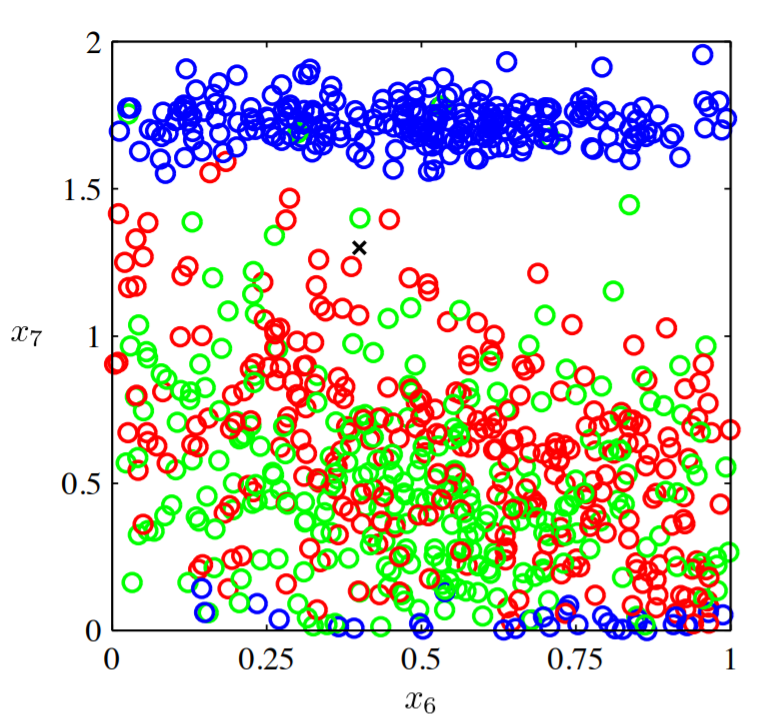
\includegraphics[scale=0.4]{03_decision_theory/02_img/continuous_data}
	\end{figure}
\end{frame}


% Section: Wrap-Up
%______________________________________________________________________
\section{Wrap-Up}
\makedivider{Wrap-Up}

% Subsection: Summary
% --------------------------------------------------------------------------------------------------------
\subsection{Summary}

% Summary
\begin{frame}{Summary}{}
	\begin{itemize}
		\item Statistical methods assume that the process that `generates' the data is 
			\textbf{governed by the rules of probability}
		\item We need class \textbf{conditional probabilities} and \textbf{class priors}
		\item Use \textbf{Bayes' theorem} to get the \textbf{class posteriors}
		\item \textbf{Bayes' optimal classifier:} Decide for the most probable class
		\item Na\"{i}ve Bayes assumes all \textbf{features to be pairwise conditionally independent}
		\item \textbf{Error minimization is not equal to risk minimization}
	\end{itemize}
\end{frame}


% Subsection: Self-Test Questions
% --------------------------------------------------------------------------------------------------------
\subsection{Self-Test Questions}

% Self-Test Questions
\begin{frame}{Self-Test Questions}{}\important
	\begin{enumerate}
		\item What are class conditional probabilities?
		\item What does \textit{Bayes optimal} mean?
		\item How can we incorporate prior knowledge about the class distribution into the classification?
		\item What is the na\"{i}ve assumption which na\"{i}ve Bayes makes? When is this a problem?
		\item Explain what maximum aposteriori is!
		\item What is misclassification and risk? Are they the same?
	\end{enumerate}
\end{frame}


% Subsection: Lecture Outlook
% --------------------------------------------------------------------------------------------------------
\subsection{Lecture Outlook}

\begin{frame}{What's next...?}{}
	\makeoverview{4}
\end{frame}


% Subsection: Recommended Literature and further Reading
% --------------------------------------------------------------------------------------------------------
\subsection{Recommended Literature and further Reading}

% Literature
%______________________________________________________________________
\begin{frame}{Recommended Literature and further Reading}{}
	\footnotesize
	\begin{thebibliography}{2}
		\literature{book}{Bishop.2006}{[1] Pattern Recognition and Machine Learning}
			{Christopher Bishop. Springer. 2006.}{$\rightarrow$ \href{
				http://users.isr.ist.utl.pt/~wurmd/Livros/school/Bishop\%20-\%20Pattern\%20Recognition\%20And\%20Machine\%20Learning\%20-\%20Springer\%20\%202006.pdf
			}{\linkstyle{Link}}, cf. chapter 1.5 \textit{'Decision Theory'}}
	\end{thebibliography}
\end{frame}


% Subsection: Meme of the Day
% --------------------------------------------------------------------------------------------------------
\subsection{Meme of the Day}

% Meme of the Day
\begin{frame}{Meme of the Day}{}
	\begin{figure}
		
\includegraphics[scale=0.35]{03_decision_theory/02_img/meme_of_the_day}
	\end{figure}
\end{frame}


% Thank you
%______________________________________________________________________
\makethanks

\end{document}